% ----------------------------------------------------------
% MODELAGEM E DEFINIÇÕES TÉCNICAS
% ----------------------------------------------------------
\section{Modelagem e definições técnicas}
Está seção tem por objetivo demonstrar as modelagens e padronizações utilizadas no desenvolvimento da aplicação.

\subsection{Modelo Entidade Relacionamento}

\begin{figure}[H]
	\centering 
	\caption{\label{fig:mer}Modelagem Entidade Relacionamento}
	\includegraphics[width=\textwidth]{../imagens/Mer-estagiei.png} 
	\fonte{Os autores}
\end{figure}

\subsection{Diagrama Entidade-Relacionamento}

\begin{figure}[H]
	\centering 
	\caption{\label{fig:der}Diagrama Entidade Relacionamento}
	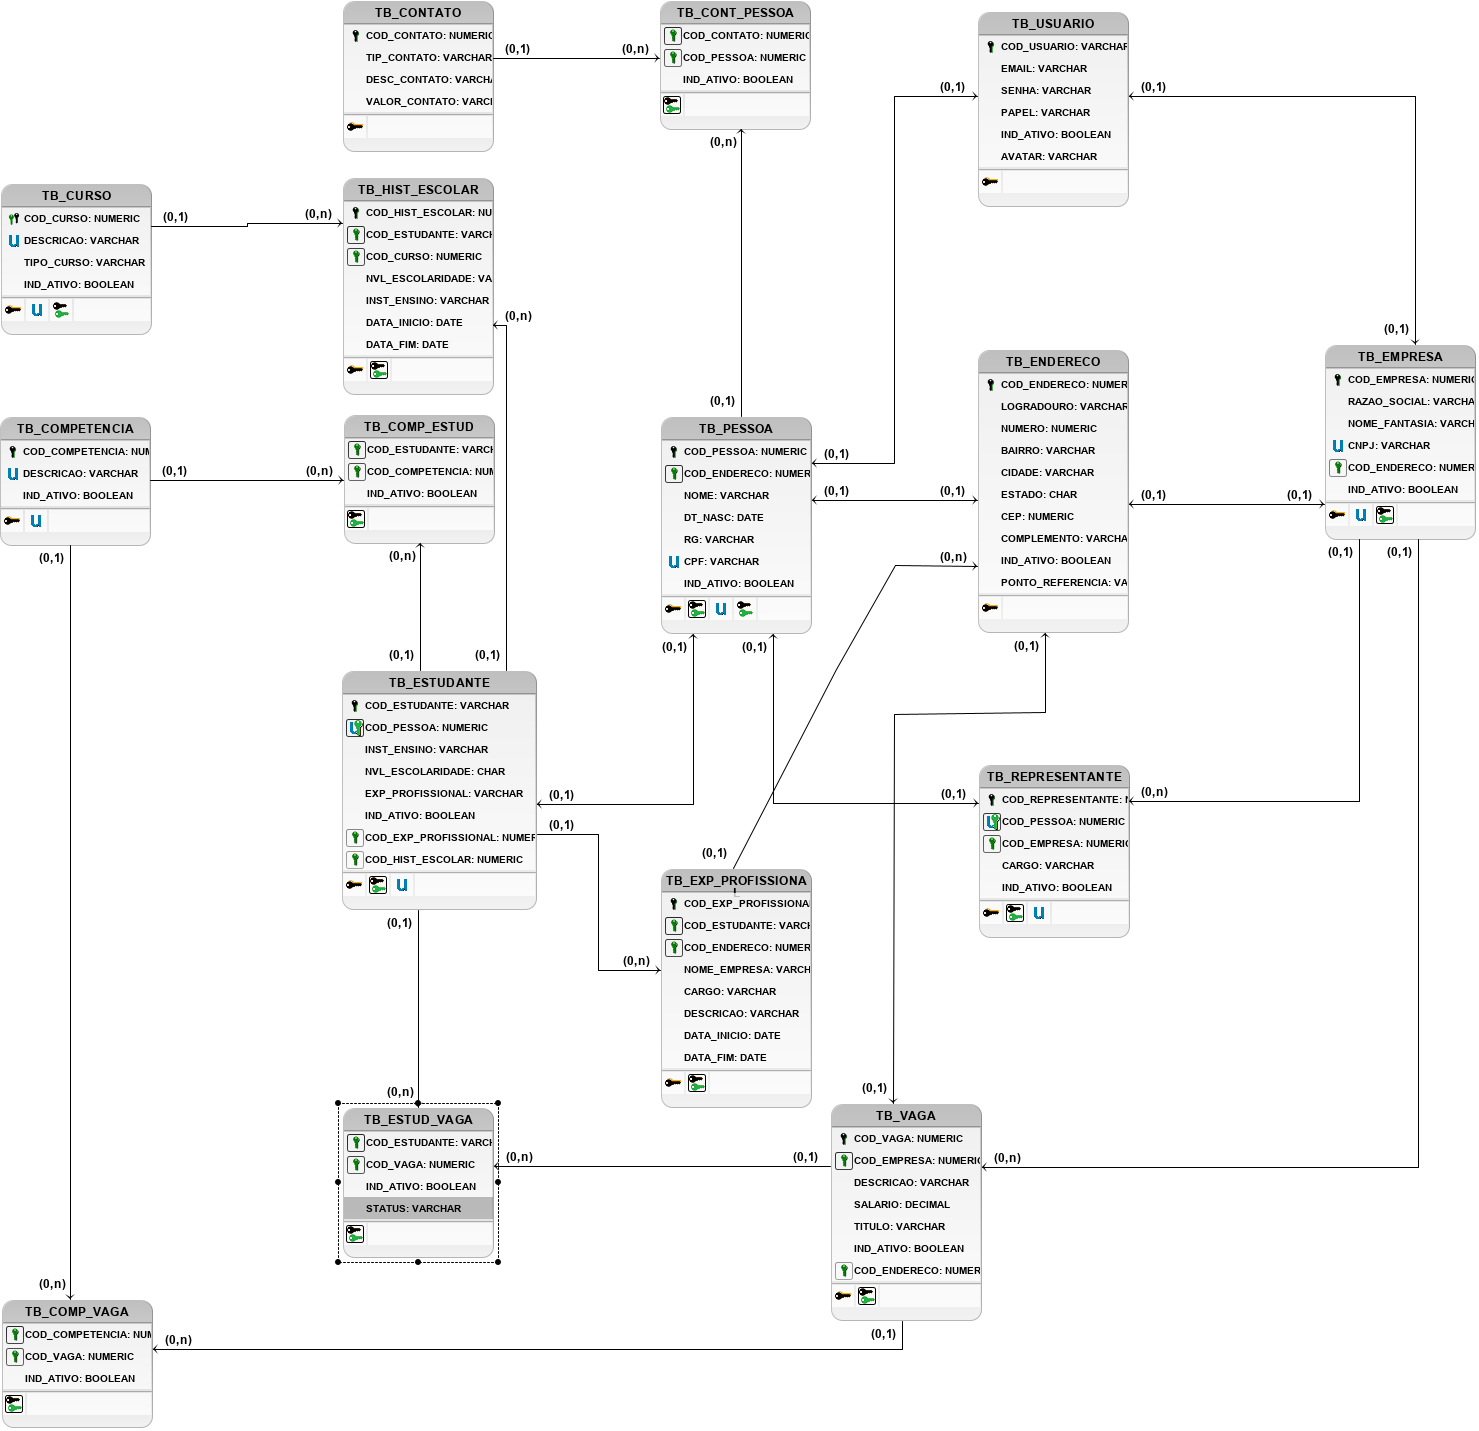
\includegraphics[width=\textwidth]{../imagens/der-estagiei.png} 
	\fonte{Os autores}
\end{figure}

\subsection{Dicionário de Dados}
A seguir mostramos as tabelas do nosso dicionário de dados.

\begin{quadro}[H]
	\caption{Legenda}
	\centering
	\begin{tabular}{| c | c |}
		\hline
		\thead{Sigla}	& \thead{Descrição}\\
		\hline
		PK			& Primary Key					\\
		\hline
		FK		& Foregin Key			\\
		\hline
		NN			& Not Null			\\
		\hline
		
		UQ			& Unique			\\
		\hline
		
		CK			& Check			\\
		\hline
		
		DEFAULT			& Default			\\
		\hline
	\end{tabular}
	\fonte{Os Autores}
	\label{Legendas}
\end{quadro}

\begin{quadro}[H]
	\caption{Campos Usuário}
	\centering
	\begin{tabular}{| c | c | c | c |}
		\hline
		\thead{Campo} & \thead{Tipo} & \thead{Restrição}	& \thead{Descrição}\\
		\hline
		Cod\_usuario & VARCHAR      & PK      & Identificador único para usuário         \\ \hline
		Senha        & VARCHAR(50)  &         & Senha de acesso                          \\ \hline
		Papel        & VARCHAR(25)  & DEFAULT & Papel de acesso do usuário no sistema    \\ \hline
		Email        & VARCHAR(50)  &         & Email de acesso                          \\ \hline
		Avatar       & VARCHAR(100) &         & Armazenamento de imagem do perfil Google \\ \hline
		Ind\_Ativo   & BOOLEAN      & DEFAULT & Indicador de estado                      \\ \hline
	\end{tabular}
	\fonte{Os Autores}
	\label{Campos Usuário}
\end{quadro}



\begin{quadro}[H]
	\caption{Campos Pessoa}
	\centering
	\begin{tabular}{| c | c | c | c |}
		\hline
		Cod\_Pessoa   & SERIAL      & PK      & Identificador único para pessoa         \\ \hline
		Cod\_Endereco & SERIAL      & FK, NN  & Chave estrangeira vinda da tb\_endereco \\ \hline
		Nome          & VARCHAR(50) & NN      & Nome                                    \\ \hline
		Dt\_Nasc      & DATE        & NN      & Data de nascimento                      \\ \hline
		RG            & VARCHAR(11) & NN      & Registro Geral                          \\ \hline
		CPF           & VARCHAR(13) & NN, UQ  & Cadastro de Pessoa Física               \\ \hline
		Ind\_Ativo    & BOOLEAN     & DEFAULT & Indicador de estado                     \\ \hline
	\end{tabular}
	\fonte{Os Autores}
	\label{Campos Usuário}
\end{quadro}

\begin{quadro}[H]
	\caption{Campos Vaga}
	\centering
	\begin{tabular}{| c | c | c | c |}
		\hline
		Cod\_Vaga     & SERIAL      & PK      & Indicador único                 \\ \hline
		Cod\_Empresa  & SERIAL      & FK NN   & Chave estrangeira da tb\_empresa  \\ \hline
		Descricao     & TEXT        &         & Descrição da vaga                       \\ \hline
		Salario       & FLOAT(5)    &         & Remuneração da vaga                     \\ \hline
		Titulo        & VARCHAR(30) &         & Titulo da vaga                          \\ \hline
		Cod\_endereco & SERIAL      & FK NN   & Chave estrangeira da tb\_endereco \\ \hline
		Ind\_Ativo    & BOOLEAN     & DEFAULT & Indicador de estado da vaga             \\ \hline
	\end{tabular}
	\fonte{Os Autores}
	\label{Campos Vaga}
\end{quadro}

\begin{quadro}[H]
	\caption{Campos Curso}
	\centering
	\begin{tabular}{| c | c | c | c |}
		\hline
		Cod\_Curso  & SERIAL      & PK      & Identificador único\\ \hline
		Descricao   & VARCHAR(50) & NN, UQ  & Descrição do curso                                            \\ \hline
		Tipo\_Curso & CHAR(1)     & NN      & Tipo do Curso) \\ \hline
		Ind\_Ativo  & BOOLEAN     & DEFAULT & Indicador de estado da tb\_curso                              \\ \hline
	\end{tabular}
	\fonte{Os Autores}
	\label{Campos Curso}
\end{quadro}

\begin{quadro}[H]
	\caption{Campos Estudante}
	
	\begin{tabular}{| c | c | c | c |}
		\hline
		Cod\_Estudante         & VARCHAR & PK         & Identificador único  \\ \hline
		Cod\_Pessoa            & SERIAL  & FK, NN, UQ & Chave estrangeira da tb\_pessoa            \\ \hline
		Cod\_Hist\_Escolar     & SERIAL  & FK, NN     & Chave estrangeira da tb\_hist\_escolar     \\ \hline
		Cod\_Exp\_Profissional & SERIAL  & FK         & Chave estrangeira  da tb\_exp\_profissional \\ \hline
		Ind\_Ativo             & BOOLEAN & DEFAULT    & Indicador de estado do estudante                 \\ \hline
	\end{tabular}
	\fonte{Os Autores}
	\label{Campos Estudante}
\end{quadro}

\begin{quadro}[H]
	\caption{Campos Empresa}
	
	\begin{tabular}{| c | c | c | c |}
		\hline
		Cod\_Empresa   & SERIAL      & PK      & Identificador único para a empresa      \\ \hline
		Razao\_Social  & VARCHAR(50) & NN      & Razão social da empresa                 \\ \hline
		Nome\_Fantasia & VARCHAR(50) &         & Nome fantasia da empresa                \\ \hline
		CNPJ           & VARCHAR(20) & NN, UQ  & Cadastro Nacional de Pessoas Jurídicas  \\ \hline
		Cod\_Endereco  & SERIAL      & FK, NN  & Chave estrangeira vinda da tb\_endereco \\ \hline
		Ind\_Ativo     & BOOLEAN     & DEFAULT & Indicador de estado da empresa          \\ \hline
	\end{tabular}
	\fonte{Os Autores}
	\label{Campos Empresa}
\end{quadro}

\begin{quadro}[H]
	\caption{Campos Representante rh}
	
	\begin{tabular}{| c | c | c | c |}
		\hline
Cod\_Representante & SERIAL      & PK      & Identificador único                \\ \hline
Cod\_Pessoa        & SERIAL      & FK, NN  & Chave estrangeira da tb\_pessoa                   \\ \hline
Cod\_Empresa       & SERIAL      & FK      & Chave estrangeira da tb\_empresa                  \\ \hline
Cargo              & VARCHAR(50) & NN      & Descrição do cargo do representante \\ \hline
Ind\_Ativo         & BOOLEAN     & DEFAULT & Indicador de estado do representante                    \\ \hline
	\end{tabular}
	\fonte{Os Autores}
	\label{Campos Representante rh}
\end{quadro}


\subsection{Endpoints da API}
%Endpoints -> \Glspl{endpoint}
%API -> \gls{api} ; APIs -> \glspl{api}
A seguir listamos os \glspl{endpoint} mapeados até o momento, com seus respectivos métodos de requisição \gls{http}.

\begin{quadro}[H]
	\caption{\Glspl{endpoint} da \gls{api}}
	\centering
	\begin{tabular}{| c | c | c |}
		\hline
		\thead{Classe Java}	& \thead{Método}	& \thead{Endpoint}		\\
		\hline
		LoginController			& POST				& /api/loginEstudante	\\
		\hline
		EstudanteController		& GET				& /api/estudante/\{id\}	\\
		\hline
		VagaController			& GET				& /api/vaga				\\
		\hline
	\end{tabular}
	\fonte{Os Autores}
	\label{endpoints}
\end{quadro}


\subsection{Listagem das Competências}
A seguir apresentamos as competências parametrizadas a fim de realizar a recomendação de vagas para os estudantes de acordo com seu perfil.

\begin{itemize}
	\label{softskills}
	\item Adaptação
	\item Atitude positiva
	\item Autoconfiança
	\item Autogestão
	\item Boa escrita
	\item Capacidade de resolver problemas
	\item Capacidade de tomar decisões
	\item Coaching
	\item Colaboração
	\item Comunicação
	\item Conhecimento político e cultural
	\item Criatividade
	\item Desenvolvimento da esquipe
	\item Desenvolvimento pessoal
	\item Empatia
	\item Estabelecimento de confiança
	\item Ética no trabalho
	\item Flexibilidade
	\item Gerenciamento de conflitos
	\item Honestidade
	\item Influência
	\item Inteligência emocional
	\item Interesse em aprender
	\item Liderança
	\item Motivação
	\item Organização
	\item Pensamento crítico
	\item Poder de negociação
	\item Proatividade
	\item Relacionamento interpessoal
	\item Resiliência
	\item Trabalho em Equipe
	\item Trabalho sob pressão
\end{itemize}